% !TEX encoding = UTF-8 Unicode
% !TeX TS-program = xelatexmk

\documentclass[a4paper,11pt, oneside]{report}

% INCLUDES

\usepackage{ifxetex, amssymb, amsmath, xfrac}

\ifxetex
	\usepackage{mathspec, unicode-math, polyglossia}
	\setdefaultlanguage{english}
	\defaultfontfeatures{Scale=MatchLowercase,Mapping=tex-text}
	\setmainfont[Ligatures={Common,TeX}]{Linux Libertine O}
	\setmathfont[vargreek-shape=unicode]{Asana Math}
	\setmonofont{Menlo}
	\newfontface\nicecal{cmsy10}
	\renewcommand{\mathcal}[1]{\text{\nicecal #1}}
\else
	\usepackage{libertine}
	\usepackage[scaled]{beramono}
	\usepackage[T1]{fontenc}
\fi

\usepackage{hyperref, listings, cite, vubtitlepage, fancyhdr, graphicx}


% hyperref setup, no ugly borders
\hypersetup{%
    pdfborder = {0 0 0}
}



% bold image caption labels without colons
\usepackage[labelsep=space, labelfont=bf]{caption}

% see notation.sty, theorems.sty and code.sty in the source folder
\usepackage{notation, theorems, code}


\maketheorem[chapter]{definition}{Definition}
\maketheorem[chapter]{lemma}{Lemma}
\maketheorem[chapter]{example}{Example}
\maketheorem{postulate}{Postulate}


% CUSTOM COMMANDS
\newcommand{\code}[1]{\texttt{#1}}
\newcommand{\concept}[1]{\emph{#1}}
\newcommand{\acro}[1]{\textsc{#1}}
\newcommand{\dutch}[1]{\textsl{#1}}

\newcommand{\strongpar}{\medskip\par}
\newcommand{\proofstep}[1]{\par\noindent\emph{#1}}

%\usepackage{pdfcomment}
%\let\comment\pdfcomment


% META
\author{\Large Klaas Moerman}
\title{\LARGE \bf Multilinear~Algebra for Multicore~Architectures \\
	                   a Case~Study in Parallel Quantum~Virtualization}

\faculty{{\bf Faculty of Sciences}}
\advisors{dr.\ Yves Vandriessche}
\advisortitle{Advisor}
\department{Department of Computer~Science \\ and Applied Computer~Science}
\reason{Bachelor Paper}
\date{June 2013}

% DOCUMENT
\begin{document}

\maketitlepage

% FRONT MATTER
\pagestyle{plain}
\pagenumbering{roman}


\clearpage
\setcounter{page}{1}
\tableofcontents
\clearpage

% MAIN MATTER
\pagestyle{fancy}
\lhead{\nouppercase{\rightmark}}
\rhead{\nouppercase{\leftmark}}
\renewcommand{\chaptermark}[1]{\markboth{#1}{}}
\renewcommand{\sectionmark}[1]{\markright{{\bf \thesection.\ #1}}}
\pagenumbering{arabic}

%% CHAPTER INTRODUCTION
\chapter{Introduction}
This document reports on an educational research project, required by the \dutch{Vrije Universiteit Brussel} to obtain a Bachelor's Degree in Computer Science.


As an introductory chapter, we present a brief overview of the \concept{quantum computing} and \concept{multicore programming} domains, establishing the context of our work. Subsequently, we express the intent of our project and hint at the general approach taken.


\section{Context}
\paragraph{Quantum Computing} Since its appearance \cite{feynman82} and development \cite{deutsch85, feynman86} in physics, quantum computing has grown into a research topic in computer science and engineering. However, we can still compare the current state of this field to the pre-electronic era of classical computing; a theoretical background for quantum computers and their physical principles exists, whereas a \concept{quantum programming} paradigm has yet to emerge. This motivates research into building a quantum programming framework, which, in the absence of actual quantum computers, entails the need for simulating them.


Several competing models for quantum computing exist, often representing radically different ways of achieving quantum computations. The low-level \concept{circuit model}, commonly used to express quantum computation \cite{nielsen-chuang, kaye-laflamme-mosca}, lacks conceptual abstraction and requires intimate knowledge of quantum mechanics. Conversely, more formal approaches at a higher level \cite{selinger-valiron, grattage} lack a low-level execution model. 


A more recent model, \concept{measurement calculus} (\acro{mc}) \cite{danos}, combines the desirable properties of high-level expressiveness and formal low-level operational semantics, meeting the requirements \cite{bettelli} for a practical quantum architecture \cite{vandriessche}. The model provides a modular and compositional abstraction for quantum programs based on a small set of primitives, it formalizes a physically realistic model for performing measurement based quantum computations and, finally, it separates the quantum and classical state of a program, yielding the realistic vision of a quantum computer as a coprocessor to a traditional \acro{cpu}, similar to \acro{gpu}s nowadays. From a computer scientists' perspective, the \acro{mc} can serve as an assembly language for quantum computers.


\paragraph{Multicore programming} As hardware engineers reach the performance limits of single core processors, multicore processors have become a mainstream commodity. This trend has considerable implications for the software community; hardware improvements no longer induce a performance gain in traditionally sequential programs, requiring a shift towards parallel programs \cite{sutter-lunch}. Moreover, the traditional concurrency primitives (coarse-grained threads) used in parallel programming show scaling issues, both from a software engineering and performance perspective, as threads prove notoriously hard to deal with (in terms of understandability, predictability and determinism) and don't yield the desired speedup due to load imbalance, synchronization, and communication \cite{lee}. Consequently, the field of parallel computing has regained its status as a research topic \cite{berkeley}.


Additionally, as microprocessor speed exceeds \acro{dram} memory speed\cite{wulf-mckee}, memory traffic strongly constrains application performance\cite{patterson}. The addition of multiple cache levels mitigates this problem, which occurs outside of the multicore realm as well. However, this \concept{memory wall} effectively prevents the scalability of multicore architectures, inciting research into new architectural solutions \cite{sutter-jungle}.


This situation, commonly dubbed \emph{the end of the free lunch} \cite{sutter-lunch}, will require new programming paradigms and languages, with fine-grained parallelism and higher flexibility \cite{sutter-larus}. In addition to classic threading libraries like \code{Pthreads} and \code{OpenMP}, solutions that existed in the \concept{high-performance computing} domain before the current multicore period, for example the \code{Cilk} \cite{cilk} or \code{NESL} \cite{nesl} languages, now become mainstream in the form of vendor libraries or frameworks such as \code{Intel Cilk++}, \code{Intel Array Building Blocks} or \code{Intel Threading Building Blocks}.


\section{Problem statement}
Vandriessche \cite{vandriessche} presented a framework for quantum programming in a layered architecture for composing and executing quantum programs. Ultimately, this framework compiles a quantum program down to a series of assembly language instructions based on the \acro{mc}. In turn, a \concept{quantum virtual machine} (\acro{qvm}) interprets and executes these instructions. The \acro{qvm} currently implements sequential interpreter with \code{libquantum} \cite{libquantum} as a back-end, however, for research purposes in quantum programming, this sequential interpreter performs poorly. The resurgence of parallel computing and the commercial availability of multicore hardware allow us to build a parallel implementation, bringing a better performing \acro{qvm} to off-the-shelf desktop computers.  However, the available development and analysis tools can only deal with the complexity of parallel programming to a limited extent, and often induce runtime overhead cancelling the parallel benefit. Thus, when aiming at \emph{optimal performance}, meaning efficient usage of the available computing resources, including memory, bandwidth, caches, processing time and active cores, the transformation form sequential to parallel turns out non-trivial.

\section{Approach}
Each quantum operation in the \acro{mc} corresponds to a large matrix operation. By carefully exploring the mathematical properties of its linear algebra formulation, in particular the \concept{tensor product}, we will obtain vector operations, reducing the workload and better matching the constraints of a multicore platform. As an implementation basis, we use an openly available parallel runtime library (Intel TBB), allowing relatively straightforward parallel code. We will validate our design decisions both theoretically and experimentally, primarily aiming at a scalable implementation of a \concept{parallel quantum virtual machine} (\acro{pqvm}).


%% CHAPTER QOPS AND MC
\chapter{Quantum Operators in the Measurement Calculus}\label{chp:qop-mc}
Before presenting the parallel adaptation of the \acro{qvm}, we must first understand the mathematical properties of its underlying operations. In the ensuing chapter, we assume a basic understanding of linear algebra, specifically \concept{linear operators} and \concept{vector spaces}. We will first introduce the foundations of quantum computing, based on the formulation in \cite{kaye-laflamme-mosca}. In the subsequent sections we describe the actual \acro{mc} primitives, constructing a formulation that can serve as an implementation basis.


%Although we would generally encourage a mathematical appetite, we do not require it and will use visual patterns illustrating the \acro{mc} operations, parallel to the linear algebra formulation. The ability to understand the \acro{mc} primitives without an extensive background in mathematics or physics illustrates its potential as an assembly language and hardware abstraction fit for computer scientists, rather than as mere mathematical machinery.


\section{Quantum Computing}
Newton's laws, or equivalently, the formalisms of Lagrange or Hamilton, form an axiomatic foundation for the class of physical theories known as \concept{classical mechanics}. Continuum mechanics, for instance, extends the basic mechanical axioms with the assumption of continuous matter, modelling the behavior of solids and fluids under stress.


Similarly, theories of \concept{quantum mechanics} share an abstract set of postulates, first formulated in their current form by Dirac and Von Neumann. As computer scientists, we can interpret these postulates as a theoretical \concept{framework} from which we can derive a quantum theory of \concept{computation}, just as the Church-Turing thesis provides a theoretical basis for classical computation. Indeed, Deutsch \cite{deutsch85} formulated a physical alternative of the Church-Turing thesis, thus suggesting a quantum mechanical foundation for computation.


We will now state the quantum mechanical postulates and construct the basic abstractions for our quantum computational model. The inquisitive reader will find a comprehensive survey of quantum computing and its history in the listed references \cite{nielsen-chuang, kaye-laflamme-mosca}.


\postulate[State space.] A unit vector in a complex Hilbert $\hilbert$ space completely defines the state of an isolated quantum system. We call this vector the \concept{state vector}, and $\hilbert$ its associated \concept{state space}.


\strongpar
As the basic building block of quantum information, analogous to its classical counterpart, the \concept{bit}, we define a \concept{qubit}~$\ket \psi$ as a vector in the two-dimensional complex vector space $\complex^2$. For an appropriate basis~$\{\ket 0, \ket 1 \}$, we have
\begin{equation}\label{eq:qubit}
\ket \psi = \alpha \ket 0 + \beta \ket1
\end{equation}
Specifically, we refer to the orthonormal basis 
\begin{equation}\label{eq:comp-basis}
\cbasis = \left\{\colvec 2 1 0, \colvec 2 0 1 \right\}
\end{equation}
as the \concept{computational basis} and write
$$\ketb 0 = \colvec 2 1 0 \quad \text{and} \quad \ketb 1 = \colvec 2 0 1$$
The unit condition of a state vector requires
$$\braket{\psi | \psi} = 1$$
from which we derive the normalization constraint on $\alpha$ and $\beta$
$$|\alpha| ^2 +|\beta|^2= 1$$


\postulate[Time evolution.]\label{thm:post-time} Any time evolution of a closed quantum system corresponds to the application of a unitary transformation $U$ to that system. Thus, for an initial state $\ket \psi$ and an evolved state $\ket \phi$, we have
$$\ket \phi = U\ket\psi$$

\lemma \label{thm:unitary-inner} {\it All and only the unitary operators preserve the inner product.}
$$\braket{U\psi , U\phi} = \braket{\psi , \phi} \Longleftrightarrow UU^\dagger = I $$
\proof A direct proof based on the associativity of linear operators.
\begin{eqnarray*}
	\braket{U\psi , U\phi} &=& \Big(\bra \psi U^\dagger\Big) \cdot \Big(U \ket \phi\Big) \\
	     &=& \bra \psi U^\dagger U \ket\phi \\
	     &=& \bra \psi I \ket \phi \\
	     &=& \bra \psi\ket \phi \\
	     &=& \braket{\psi, \phi}
\end{eqnarray*}

\strongpar
Lemma \ref{thm:unitary-inner} establishes the importance of unitary operators, as the only norm-preserving operators. Using the computational basis \eqref{eq:comp-basis}, we can express a qubit operator\footnote{The quantum computing literature often refers to qubit operators as \concept{gates}, in the context of \concept{quantum circuits}. In this report, adhering to the measurement calculus' standards, we avoid such terminology.} $U$ as a $\complex^{2 \times 2}$ matrix. For example, the $X$~operator, the quantum analogy of the classical \acro{not} bit-operation, acts on the basis vectors as
$$X: \complex^2 \to \complex^2 :
\left\{\begin{alignedat}{2}
     	      \ketb 0 & \mapsto \ketb 1\\
	      \ketb 1 & \mapsto \ketb 0
\end{alignedat} \right.$$
and has the matrix representation
$$X = \X$$
Recall from linear algebra that the action on the basis vectors completely specifies a linear operator; $X$ therefore maps a qubit $\ket \psi = \alpha\ketb 0 + \beta\ketb 1$ to
$$X\ket \psi = \alpha \ketb 1 + \beta \ketb 0$$


\postulate[Composition of systems.]\label{thm:post-compose} The state vectors $\ket {\psi_1}$ and $\ket{\psi_2}$ of two systems in their respective state spaces $\hilbert_1$ and $\hilbert_2$ determine the state vector $\ket {\psi_1} \otimes \ket {\psi_2}$ of the combining system in state space $\hilbert_1 \otimes \hilbert_2$.


Inductively applying this postulate shows that the composition of $n$ subsystems in state $\ket{\psi_i} \in \hilbert_i$ will result in the state vector $\bigotimes_i \ket{\psi_i} \in \bigotimes_i\hilbert_i$, where $i \in \{1, 2, \dots, n\}$.


\strongpar
Continuing the analogy with classical bits, we call the composition of $n$ qubits $\ket {\psi_i}$ a \concept{quregister}, with state vector
\begin{equation}\label{eq:qureg-tensor}
\ket \psi = \Tensor{i}\ket{\psi_i}
\end{equation}
in state space $$\hilbert = \left(\complex^2\right)^{\otimes n} = \complex^{2^n}$$


When manipulating a quregister, we cannot always decompose it back into the tensor product of its constituent qubits (in the form of equation \eqref{eq:qureg-tensor}). We call a quregister \concept{separable} if we can express it as a tensor product of individual qubits, conversely, we call a quregister \concept{entangled}, when we cannot decompose it into a tensor product. In general, the set of $2^{n}$-dimensional state vectors formed by taking the tensor product of two $2^{n-k}$-dimensional state vectors contains only a sparse subset of all the possible $2^{n}$-dimensional state vectors \cite{kaye-laflamme-mosca}.


\example No combination of coefficients $\alpha_0$, $\alpha_1$ and $\beta_0$, $\beta_1$ exists such that the 2-qubit state
$\ket \psi =  {1 \over \sqrt{2}}\ketb{00} + {1 \over \sqrt{2}}\ketb{11}$ equals the tensor decomposition $(\alpha_0\ketb0+\alpha_1\ketb1) \otimes ( \beta_0\ketb0 + \beta_1\ketb1 )$.


\proof[By contradiction.] Assume the existence of such coefficients $\alpha_0$, $\alpha_1$, $\beta_0$, $\beta_1$ and consider the resulting vectors
$$
\ket \psi = {1 \over \sqrt2}\colvec 4 1 0 0 1 \quad \text{and} \quad \colvec 4 {\alpha_0\beta_0} {\alpha_0\beta_1} {\alpha_1\beta_0} {\alpha_1\beta_1} 
$$
By the first and the last rows, we must refute that any of the coefficients equal zero. However, by the second and third rows, we must conclude that at least two of the coefficients equal zero. This contradiction implies that no such coefficients can exist.

\postulate[Measurement.] 
For a given orthonormal basis $\{\ket {\phi_i}\}$ of a state space $\hilbert$, one can perform a \concept{Von Neumann measurement} of a state $\ket \psi = \sum_i\alpha_i\ket{\phi_i}$, which outputs a label $i$ with probability $\alpha_i^2$ and leaves the system in state $\ket{\phi_i}$.

Note that for the state $\ket \psi$ and basis vector $\ket{\phi_i}$, the amplitude $\alpha_i$ equals
\begin{equation}
\alpha_i = \braket{\phi_i | \psi}
\end{equation}

\section{Computational Basis}
At its core, a \acro{qvm} requires implementing unitary operators on vectors in a complex Hilbert space. To perform actual calculations, we need to choose a basis for this vector space. This basis, called the \concept{computational basis}, will remain implicit throughout this report.


\definition For the complex vector space $\complex^2$, we define the computational basis $\cbasis$ as the set of colums of $I$, the unit matrix.
\begin{equation}
\cbasis = \Set{\colvec 2 1 0, \colvec 2 0 1}
\end{equation}
We use the compact Dirac notation
\begin{equation}
\ketb 0 = \colvec 2 1 0 \quad \text{and} \quad \ketb 1 = \colvec 2 0 1
\end{equation}
We can express a qubit $\ket \psi \in \complex^2$ as a linear combination of these basis vectors
$$\ket \psi = \colvec 2 \alpha \beta = \alpha \ketb 0 + \beta \ketb 1$$


\definition[Computational basis.] We define the computational basis $\cbasis_n = \cbasis^{\otimes n}$ spanning the complex vector space $\hilbert = \complex^{2^n}\!\!$ as the set of columns of the unit matrix~$I^{\otimes n}$
\begin{equation}
\cbasis_n = \cbasis^{\otimes n} = \Set{\ketb 0, \ketb 1}^{\otimes n}  = \Set{ \colvec 6 1 0 0 \vdots 0 0, \colvec 6 0 1 0 \vdots 0 0, \; \dots \;, \colvec 6 0 0 0 \vdots 0 1 }
\end{equation}
We make extensive use of Iverson's bracket notation \cite{knuth-graham-patashnik}, mapping a true statement to 1 and a false statement to 0. Combining Dirac notation and Iverson brackets, we obtain a more compact representation for a basis vector
$$
\ket i = \colvec 3 {\ive{i = 0}} \vdots {\ive{i = 2^n-1}} \qquad 0 \leqslant i < 2^n
$$
With respect to this basis, we can express the $n$-qubit quregister $\ket \psi$ as the linear combination
\begin{equation}
\ket \psi = \Sum{i} \alpha_i \ket i
\end{equation}
We call $\alpha_i$ the \concept{probability amplitude} of $\ket i$ in $\ket \psi$. 


\example To show the relation between column vector (unary) and Dirac notation (binary or decimal), let us consider the state space of 2-qubit quregisters, which has four basis vectors
\begin{align*}
\ket 0 &= \ketb 0 \otimes \ketb 0 = \ketb{00} = \colvec 4 1000 & \ket 2 = \ketb 1 \otimes \ketb 0= \ketb {10} = \colvec 4 0010 \\
\ket 1 &= \ketb 0 \otimes \ketb 1 = \ketb {01} = \colvec 4 0100 & \ket 3 =  \ketb 1 \otimes \ketb 1 = \ketb {11} = \colvec 4 0001 
\end{align*}
The {\tt binary} notation has our preference, as the number of qubits in the quregister corresponds to the number of digits in the ket; the decimal notation lacks this property.
Given two qubits (using subscript to identify the qubit and the superscript to identify the basis vector)
$$ \ket{\psi_1} = \psi_1^\bin 0 \ketb0 + \psi_1^\bin 1 \ketb1
 \quad\text{and}\quad \ket{\psi_2} = \psi_2^\bin 0 \ketb0 + \psi_2^\bin 1\ketb1$$
the combining quregister $\ket \psi = \ket \psi_1 \otimes \ket \psi_2$ becomes
\newcommand{\coef}[2]{\psi_{#2}^{\bin{#1}}}
$$\ket \psi =   \coef 0 1 \coef 0 2 \ketb{00} + \coef 0 1 \coef 1 2\ketb{01}
                 + \coef 1 1 \coef 0 2 \ketb{10} + \coef 1 1 \coef 1 2\ketb{11}$$


The example above reveals some inherently binary properties of the computational basis and the tensor product. While familiar to the seasoned computer scientist, we will develop these properties independently of integer representation and bitwise operations, maintaining mathematical rigor and providing a concise notation connecting the linear algebra formulation and the actual \acro{qvm} implementation.


\definition[Generalized parity.] Consider a non-negative integer and its canonical binary representation\footnote{The least significant bit resides at position zero. The common two's complement representation would qualify.}. We call this number $k$-odd when the bit at position $k$ equals $\bin 1$ and  $k$-even when the bit equals $\bin 0$. The function $\parity_k$ maps $k$-odd numbers to $1$  and $k$-even numbers to $0$.
\begin{equation}\label{eq:odd-even}
\begin{array}{rccl}
\parity_k : & \naturals & \to & \integer_2 \\
                 &  n & \mapsto & n \backslash 2^k \bmod 2
\end{array}
\end{equation}
where $a \backslash b = \floor{{a \over b}}$ denotes integer division. The reader may recognize the composition of a bit shift and a bit test operation. The base case $\parity_0$ degenerates into a simple parity test, mapping odd numbers to~$1$ and even numbers to~$0$.

\example Calculate $\parity_k(13)$ for $k\in\{0,1,2,3\}$
\begin{align*}
\parity_0(13) &= 13 \backslash 2^0 \bmod 2 & \quad\parity_2(13) &= 13 \backslash 2^2 \bmod 2  \\
     &= 1                                               &&=1 \\
     &&&\\
\parity_1(13)
     &= 13 \backslash 2^1 \bmod 2 &\quad\parity_3(13) &= 13 \backslash 2^3 \bmod 2 \\
      &= 0                                           &&= 1
\end{align*}
This corresponds to the binary representation $13 = \bin{1101}$. Note that $\parity_k$ will correctly extend the binary numeral with zeros, for example $$\parity_4(13) = {13 \backslash 2^4} \bmod 2 =0$$

%\comment{include graph of Pk for several k}

We prove some useful properties of this function, which we rely on for developing our implementation. These properties should come as no surprise when interpreting $\parity_k(n)$ as function returning the bit  at position $k$ of integer $n$.

\lemma The generalized parity function $\parity_k(n)$ has a period $p_k = 2^{k+1}$.
\proof[By direct calculation.]
\begin{equation*}
\begin{split}
\parity_k(n + p_k)
    &= \floor{{n + 2^{k+1} \over 2^k}} \bmod 2 \\
    &= \floor{{n \over 2^k} + 2} \bmod 2 \\
    &= \left(\floor{{n \over 2^k}} \bmod 2\right) + (2 \bmod 2) \\
    &= \parity_k(n) + 0 = \parity_k(n)
\end{split}
\end{equation*}

\lemma Within a single period $p_k = 2^{k+1}$, $\parity_k$ equals $0$ in the first half and $1$ in the second half. We call the half-period $b_k = 2^k$ the even \concept{block} and the second half the odd \concept{block}. Symbolically
\begin{equation}\label{eq:stride}
\forall \lambda \in \naturals: \left\{\begin{alignedat}{2}
&\parity_k(2\lambda b_k + \sigma) =  0  \\
&\parity_k((2 \lambda + 1) b_k + \sigma) = 1
\end{alignedat}\right. \qquad\text{where}\quad 0 \leqslant \sigma < b_k 
\end{equation}
\proof[By direct calculation.] We prove only the first equation of \eqref{eq:stride}, the second follows by analogy.
\begin{equation*}
\begin{split}
\parity_k(2\lambda b_k + \sigma)
  &= \floor{{2\lambda 2^k + \sigma \over 2^k}} \bmod 2 \\
  &= \floor{2\lambda + {\sigma \over 2^k}} \bmod 2
\end{split}
\end{equation*}
because $\lambda \in \naturals$ and $\sigma < 2^k$, we find
\begin{equation*}
\begin{split}
\parity_k(2\lambda b_k + \sigma)
  &= 2\lambda \bmod 2 \\
  &= 0
\end{split}
\end{equation*}


\section{Positional Operators}
As established by Postulate \ref{thm:post-time}, the application of a unitary operator to a quantum state results in an evolved quantum state. These unitary operators will form the basis of quantum computations. We define a class of operators on quregisters, describing the application of an operator to one of its qubits.
%\comment{add short introduction to operators on qubits before generalizing to quregisters}
\definition[Positional operator.] \label{thm:def-qop} For any unitary operator $U\!:\complex^2 \to\complex^2$, we define the positional operator~$U_t\!:\hilbert\to\hilbert$ as
\begin{equation} \label{eq:qop}
U_t = \Tensor{i}U^\ive{i=t}
\end{equation}
We prove the following lemma, ensuring the unitarity of a positional operator.
\lemma Two unitary operators $A$ and $B$  have a unitary tensor product.
\proof We must show that the tensor product $A \otimes B$ satisfies the definition of a unitary operator $UU^\dagger = I$
\begin{equation*}
\begin{split}
(A \otimes B)(A \otimes B)^\dagger
     &= (A \otimes B)(A^\dagger \otimes B^\dagger) \\
     &= AA^\dagger  \otimes BB^\dagger
     \end{split}
\end{equation*}
Indeed, for unitary $A$ and $B$, we find (omitting the dimensions of the identity)
$$(A \otimes B)(A \otimes B)^\dagger  = I \otimes I = I$$


\example \label{thm:ex-x3} Consider the $X$ operator $\smat{0 & 1 \\ 1 &0}$. The positional operators $X_2$ and $X_3$ on a quregister $\ket \psi$ of 3 qubits become
\begin{align*}
X_2 &= I \otimes X \otimes I &&& X_3 &= I \otimes I \otimes X \\
 &= \I \otimes \X \otimes \I & &&     &= \I \otimes \I \otimes \X \\
   & = \mat{
       0 & 0 & 1 & 0 & 0 & 0 & 0 & 0 \\
       0 & 0 & 0 & 1 & 0 & 0 & 0 & 0 \\
       1 & 0 & 0 & 0 & 0 & 0 & 0 & 0 \\ 
       0 & 1 & 0 & 0 & 0 & 0 & 0 & 0 \\ 
       0 & 0 & 0 & 0 & 0 & 0 & 1 & 0 \\
       0 & 0 & 0 & 0 & 0 & 0 & 0 & 1 \\
       0 & 0 & 0 & 0 & 1 & 0 & 0 & 0 \\ 
       0 & 0 & 0 & 0 & 0 & 1 & 0 & 0 }
 &&&
       &= \mat{
       0 & 1 & 0 & 0 & 0 & 0 & 0 & 0 \\
       1 & 0 & 0 & 0 & 0 & 0 & 0 & 0 \\
       0 & 0 & 0 & 1 & 0 & 0 & 0 & 0 \\ 
       0 & 0 & 1 & 0 & 0 & 0 & 0 & 0 \\ 
       0 & 0 & 0 & 0 & 0 & 1 & 0 & 0 \\
       0 & 0 & 0 & 0 & 1 & 0 & 0 & 0 \\
       0 & 0 & 0 & 0 & 0 & 0 & 0 & 1 \\ 
       0 & 0 & 0 & 0 & 0 & 0 & 1 & 0 }
\end{align*}


\strongpar
Consider the tensor product's mixed product property
$$(A\otimes B)(C \otimes D) = (AC \otimes BD)$$
For a quregister in a separable state, we can distribute $U_t$ over the individual qubits
$$U_t \ket \psi = \left(\Tensor{i}U^\ive{i=t}\right) \left(\Tensor{i}\ket{\psi_i}\right) = \Tensor{i}\left(U^\ive{i=t}\ket {\psi_i}\right)$$
applying the operator $U$ to qubit $\ket {\psi_t}$ and the identity $I$ to the others.


\example \label{thm:ex-x3-sep} The application of $X_3$ on a separable $\ket \psi$ of three qubits $\ket {\psi_i} = \smat{\alpha_i \\ \beta_i}$ applies $X$ to the third qubit
\begin{equation*}
\begin{split}
X_3\ket \psi &= \left( X^\ive{1=3} \otimes X^\ive{2=3} \otimes X^\ive{3=3} \right) \left( \ket{\psi_1} \otimes \ket{\psi_2} \otimes \ket{\psi_3} \right) \\
       &= \left( I \otimes I \otimes X \right) \left( \ket{\psi_1} \otimes  \ket{\psi_2} \otimes  \ket{\psi_3} \right) \\
       &= I \colvec 2 {\alpha_1} {\beta_1} \otimes I \colvec 2 {\alpha_2} {\beta_2} \otimes X \colvec 2 {\alpha_3} {\beta_3} \\
       &= \colvec 2 {\alpha_1} {\beta_1} \otimes \colvec 2 {\alpha_2} {\beta_2} \otimes  \colvec 2 {\beta_3} {\alpha_3}
\end{split}
\end{equation*}


\strongpar
In general, quantum entanglement prohibits the use of tensor decomposition to find the action of a positional operator on individual qubits. A direct matrix representation becomes unwieldy, as the number of dimensions of $\hilbert$ increases exponentially with the number of qubits. We will therefore describe positional operators as acting on the computational basis vectors, thereby obtaining a complete yet compact notation using the generalized parity function.


\lemma A basis vector $\ket i$ ($0 \leqslant i < 2^n $) has the tensor decomposition
\begin{equation}\label{eq:basis-vec}
\ket i = \Tensor{j} \ket{\parity_{n-j}(i)}
\end{equation}

Thus, we find the action of a positional operator $U_t$ on the basis
\begin{equation}\label{eq:qop-basis}
U_t \ket i = \left(\Tensor{j} U^\ive{j=t}\right)\left(\Tensor{j} \ket{\parity_{n-j}(i)}\right) = \Tensor{j} U^\ive{j=t}\ket{\parity_{n-j}(i)}
\end{equation}

\example Continuing examples \ref{thm:ex-x3} and \ref{thm:ex-x3-sep}, consider the state space $\hilbert = \complex^8$ of 3-qubit registers, and its computational basis $\cbasis_3$.
\begin{equation*}
\begin{split}
X_2\ket 0 &= X_2 \big(\ket {\parity_2(0)} \otimes \ket  {\parity_1(0)} \otimes \ket  {\parity_0(0)} \big)\\
   &= I \ketb 0 \otimes X \ketb 0 \otimes I \ketb 0       \\
   &= \ketb 0 \otimes \X \colvec 2 1 0  \otimes \ketb 0        \\
   &= \ketb 0 \otimes \colvec 2 0 1 \otimes \ketb 0      \\
   &= \ketb 0  \otimes \ketb 1 \otimes \ketb 0      \\
   &= \ket 2    \\
\end{split}
\end{equation*}
\begin{equation*}
\begin{split}
 X_3\ket 6 &= X_3 \big(\ket {\parity_2(6)} \otimes \ket  {\parity_1(6)} \otimes \ket  {\parity_0(6)} \big) \\
   &= I \ketb 1  \otimes I \ketb 1 \otimes X \ketb 0 \\
   &= \ketb 1   \otimes \ketb 1 \otimes \X \colvec 2 1 0 \\
   &= \ketb 1 \otimes \ketb 1 \otimes \colvec 2 0 1 \\
   &= \ketb 1  \otimes \ketb 1 \otimes \ketb 1 \\
   &= \ket 7 
   \end{split}
\end{equation*}

We can now fully express a quregister $\ket \psi$ as the result of the tensor product of $n$ qubits $\ket {\psi_j}= \psi_j^\bin0\ketb 0 + \psi_j^\bin1\ketb 1$ as a linear combination of the basis vectors $\ket i$
\begin{equation}\label{eq:qureg-lin-comb}
\begin{split}
\ket \psi &= \Tensor{j} \psi_j^\bin0\ketb 0 + \psi_j^\bin1\ketb 1  \\[0.1em]
   &= \Sum{i} \Product{j}\psi_j^{\parity_{n-j}(i)} \ket i
\end{split}
\end{equation}

Using equations \eqref{eq:qureg-lin-comb} and \eqref{eq:qop-basis}, we can now generally express the application of a positional operator $U_t$ on a quregister $\ket \psi$ of $n$ qubits $\ket {\psi_j}= \psi_j^\bin0\ketb 0 + \psi_j^\bin1\ketb 1$
\begin{equation}\label{eq:qop-qureg}
\begin{split}
U_t\ket\psi &= \Sum{i}\Product{j}\psi_j^{\parity_{n-j}(i)} U_t \ket i \\
 &= \Sum{i}\Product{j}\psi_j^{\parity_{n-j}(i)} \Tensor{k} U^\ive{k=t} \ket {\parity_{n-k}(i)}
\end{split}
\end{equation}
As we will see in Chapter \ref{chp:implementation}, this equation will prove useful as a basis for a parallel implementation. Before describing the actual operations in the measurement calculus, we need to construct a second class of operators.


\definition[Controlled operator.] For any unitary operator $U\!:\complex^2\to\complex^2$, we~define the controlled operator $\cU_{c,t}\!:\hilbert\to\hilbert$, acting on the computational basis $\cbasis_n$
\begin{equation}\label{cop-basis}
\cU_{c,t}\ket i = U^\prime_t\ket i\qquad\text{where}\quad U^\prime = U^{\parity_{n-c}(i)}
\end{equation}
applying a positional operator $U_t$ to all $(n-c)$-odd basis vectors and the identity to the others\footnote{Some notational ambiguity may arise. When $\parity_c(i) = 0$, the operator $U^\prime$ equals $I$, the identity; the controlled operator $\cU_{c,t}$ then becomes $I_t$. While the notation $I_t$ usually specifies the dimension $t$ of the identity $I$, we denote a positional operator applying $I$ at position $t$, resulting in an identity of dimension $2^n$, with $n$ the number of qubits. We avoid this confusion by consistently leaving the dimensions of identities implicit.}.


\example Consider a quregister $\ket \psi$ of two qubits. The controlled operator $\widehat{X}_{1,2}$ acts on the second qubit with the first as a control qubit
\begin{equation*}
\widehat{X}_{1,2} : \complex^4 \to \complex^4 : \left\{
\begin{array}{lcl}
\ket 0 \mapsto I\otimes X^{\parity_1(0)}\ket 0 = I\ketb 0 \otimes I\ketb 0\! &=& \ket 0\\
\ket 1 \mapsto I\otimes X^{\parity_1(1)}\ket 1 = I\ketb 0 \otimes I\ketb 1\! &=& \ket 1\\
\ket 2 \mapsto I\otimes X^{\parity_1(2)}\ket 2 = I\ketb 1 \otimes X\ketb 0\! &=& \ket 3\\
\ket 3 \mapsto I\otimes X^{\parity_1(3)}\ket 3 = I\ketb 1 \otimes X\ketb 1\! &=& \ket 2
\end{array} \right.
\end{equation*}


\strongpar
Analoguous to equation \eqref{eq:qop-qureg}, we use \eqref{eq:qureg-lin-comb} to obtain the application of a controlled operator $\cU_{c,t}$ to a quregister $\ket \psi$
\begin{equation}\label{eq:cop-qureg}
\cU_{c,t}\ket\psi = \Sum{i}\Product{j}\psi^{\parity_{n-j}(i)}_j \Tensor{k} U^{\ive{k=t}\parity_{n-c}(i)} \ket {\parity_{n-k}(i)}
\end{equation}


\section{Measurement calculus}
At its execution level, the measurement calculus performs three classes of operations on quregisters: \concept{entanglement}, \concept{measurement} and \concept{correction} \cite{vandriessche}. Four basic operators capture these operations.

\definition[$X$ and $Z$ operators.] The $X$ and $Z$ correction operators, sometimes called $\sigma_x$ and $\sigma_z$ \cite{kaye-laflamme-mosca}
\begin{equation}
\quad X = \X \qquad\text{and}\qquad Z=\Z
\end{equation}
From this, we can deduce their actions on the basis vectors $\ketb 0$ and $\ketb 1$
\begin{align}
X: \complex^2 \to \complex^2 :& \left\{\begin{aligned}
     	      \ketb 0 & \mapsto \ketb 1\\
	      \ketb 1 & \mapsto \ketb 0
\end{aligned} \right. \label{qop-x}
\\
Z : \complex^2 \to \complex^2 :& \left\{\begin{aligned}
     	      \ketb 0 &\mapsto\phantom{-}\ketb 0\\
	      \ketb 1 &\mapsto -\ketb 1
\end{aligned} \right. \label{eq:qop-z}
\end{align}
Using equation \eqref{eq:qop-basis} we find the corresponding positional operators, acting on a basis vector $\ket i$ as
\begin{equation}\label{qop-cz-basis}
X_t \ket i = \ket {i + \sigma_{n-t}(i)2^{n-t}}
\qquad\text{and}\qquad
Z_t \ket i = \sigma_{n-t}(i)\ket{i}
\end{equation}
where $\sigma_k(i) = (-1)^{\parity_k(i)}$ equals $-1$ for a $t$-odd $i$ and $+1$ otherwise.

\definition[Controlled $Z$ entanglement operator.] This operator entangles two qubits. Its definition follows from \eqref{eq:qop-z} and the definition of controlled operators.
\begin{equation}
\widehat{Z}_{c,t}\ket i = (-1)^{\parity_{n-c}(i) \parity_{n-t}(i)}\ket i
\end{equation}

\definition[Measurement operator.]

%% CHAPTER PLATFORM
\chapter{Implementation Platform} \label{chp:platform}
In this chapter, we explore the constraints on the \acro{qvm} implementation imposed by the targeted multicore architecture and introduce some of the available tools for developing parallel software. Furthermore, we show how to measure and analyze the results and decide on an appropriate experimental setup. To illustrate the properties of our platform, we interleave the sections of this chapter with the implementation of simple example algorithms, preluding the actual implementation process.



\section{Computational Model}
The high complexity of modern processors, especially multicore processors, makes it hard to make accurate or relevant predictions regarding algorithmic performance. The classic random access model, assuming a flat memory address space and unit-cost memory access, disregards the cache hierarchy, thereby underestimating the effect of data movement on execution speed \cite{snyder-lin, chatterjee-sen}.


Cache effects and memory bandwidth exert an even bigger influence on multicore applications \cite{snyder-lin}. When multiple processing units operate on disjoint parts of the same cache line, data might needlessly move between cache levels, a problem known as \concept{false sharing} \cite{snyder-lin, sutter-jungle}. In symmetric multiprocessors (\acro{smp}s), main-memory access of all \acro{cpu}s requires passing through the same front-side bus (\acro{fsb}). This bottleneck limits memory bandwidth, resulting in latency increasing with the number of processors\cite{drepper}. More advanced solutions attach different sections of the memory to different \acro{cpu}s, known as non-uniform memory architecture (\acro{numa}), where remote memory access comes at a higher cost than accessing local memory.


Several authors have identified \concept{dwarfs} of scientific computing: classes of applications related by similarity in operations and data movement. The dwarfs allow for capturing the common requirements of applications while remaining reasonably independent of specific implementations.\cite{berkeley}. Considering the seven dwarfs defined by \cite{berkeley}, a \acro{qvm} qualifies as a Class 3 dwarf (spectral methods), related to algorithms like Fast-Fourrier Transform \cite{frigo}. It seems tempting to situate our \acro{qvm} in Class 1 or 2 (dense or sparse linear algebra), however, we do not directly implement the linear algebra formulation of the \acro{mc}; with the benefit of foresight, we anticipate on mainly performing data permutation and very little computation. It follows that memory access patterns will determine the performance of our \acro{pqvm}.


\section{Development Tools}
The transformation of a single-threaded program into a multithreaded program requires a careful redesign. Ideally, we want to obtain a portable program\footnote{from small multicore to huge manycore machines, different memory layouts, and different cache hierarchies} while maintaining optimal performance; concretely, we need to balance programming effort and performance loss \cite{michailidis-margaritis}. Several libraries and languages for parallel programming exist, spanning different abstraction levels. 


The \acro{posix} threads library (\code{Pthreads}) provides a low level threading \acro{API}. It requires explicit control of threads, leaving the programmer with great flexibility, at the expense of high complexity of manually managing synchronization primitives, such as locks, mutexes, semaphores, barriers and condition variables \cite{michailidis-margaritis, snyder-lin}. \code{OpenMP} (\code{OMP}), a basic multithreading tool for \code{C}, \code{C++} or \code{Fortran} programs, offers some basic abstractions of threads, in the form of compiler directives (\code{pragma}) marking parallel sections or loops\cite{omp, michailidis-margaritis, snyder-lin}.

\code{Intel Cilk++}, a language based on \code{Cilk} \cite{cilk}, extends the \code{C++} language with extra keywords telling the compiler which parts to make parallel. Divide and conquer algorithms perform well in this language. Additionally, \code{Cilk++} provides some code analysis tools, e.g. for detecting race condition \cite{michailidis-margaritis}.

\code{Intel Array Building Blocks} (\code{ArBB}), designed to use the features of existing and upcoming multicore and many core processors, extends code{C++} for complex data parallelism. \code{ArBB} provides a rich set of data containers allowing high-level expression of parallel programs \cite{michailidis-margaritis}. Intel discontinued this project earlier this year \cite{intel-arbb}.

\code{Intel Threading Building Blocks} (\code{TBB}) provides task-based parallelism; hiding actual threads from the programmer, \code{TBB} provides a library allowing the programmer to formulate a parallel program at a high level of abstraction, in the form of tasks executed by its runtime environment \cite{tbb, michailidis-margaritis}.


\example We will write an example algorithm\footnote{complete source code at \url{http://github.com/kmoerman/pqvm}} with \code{TBB} to normalize vectors of real and complex numbers. For arbitrary vectors, we need a two-step process: first calculate the norm (a  reduce operation), then divide each component of the vector by this norm (a map operation). For brevity, the example below only includes the reduction step.


Using \code{TBB}'s \code{parallel\_reduce} function requires writing a class with an overloaded \code{operator()} method encapsulating the work for a certain range of the vector, and a \code{join} method combining the results of two tasks. The \code{TBB} runtime will split a given range and assign a parallel task to each of its parts, or recursively split down to an appropriate size for a parallel task \cite{tbb}.
\lstinputlisting{normalize.cpp}


\section{Testing Environment} We executed code on two testing machines, both in a standard \code{C++} environment, with \code{TBB} version 4.1. We used the first, called \code{wilma} for exploratory work, including the examples in this chapter. This machine consists of 8 processors in a shared memory architecture.
\begin{verbatim}
Intel(R) Xeon(R) CPU X5687 @ 3.60GHz GenuineIntel GNU/Linux
Linux wilma 3.2.45-wilma #1 SMP Thu May 16 13:02:41 CEST 2013 x86_64

g++ (GCC) 4.7.1, -O2 optimization level
\end{verbatim}
\begin{figure}[hbp]
	\centering
	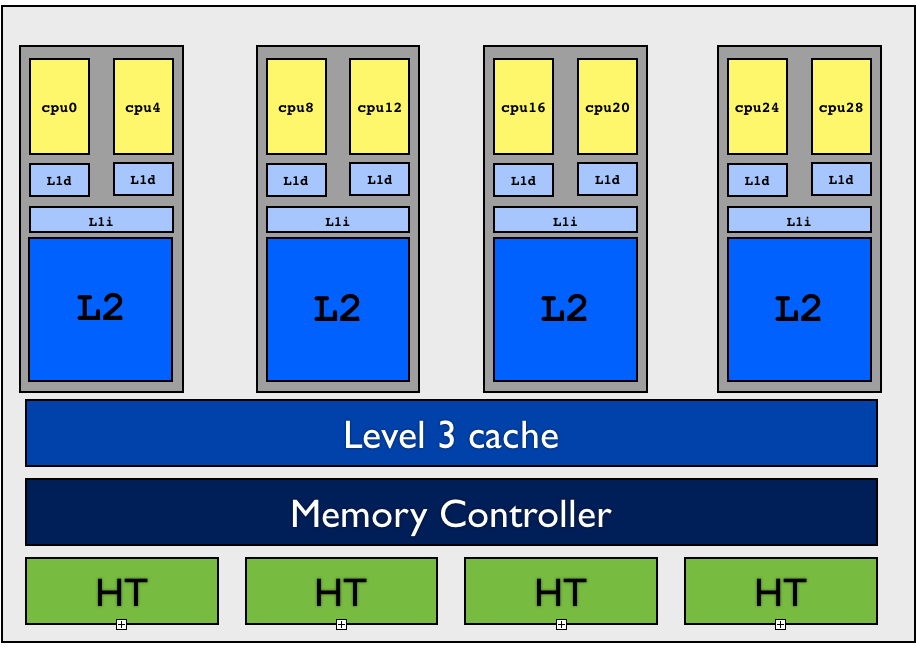
\includegraphics[width=\columnwidth]{serenity-node.png}
	\caption{Serenity node model \cite{serenity}} \label{fig:serenity-node}
\end{figure}
We used second machine, called \code{serenity}, provided by the computer science department, for the actual implementation.
\begin{verbatim}
AMD Opteron 6300 Abu Dhabi 16 core
Linux serenity 3.8.0-19-generic #29-Ubuntu SMP Wed Apr 17 18:16:28 UTC
2013 x86_64 x86_64 x86_64 GNU/Linux

g++ (Ubuntu/Linaro 4.7.3-1ubuntu1) 4.7.3, -O2 optimization level
\end{verbatim}

This machine consists of 64 processors, distributed across 8 nodes in a \acro{numa} architecture, giving each node its own memory controller. Figure \ref{fig:serenity-node} illustrates the structure of a node.

\section{Experimental Analysis}
We need to define some performance metrics for our software and hardware to allow for an objective evaluation of the results. Predominantly, we want to analyze the \concept{scaling} behavior of a parallel program. \concept{Weak scaling} characterizes the change in execution time as the problem size changes, while keeping the number of processors fixed. Conversely, \concept{strong scaling} characterizes the change in execution time as the number of processors changes, while keeping the problem size fixed.

\begin{figure}[hbp]
	\centering
	\hspace*{-0.07\columnwidth}
	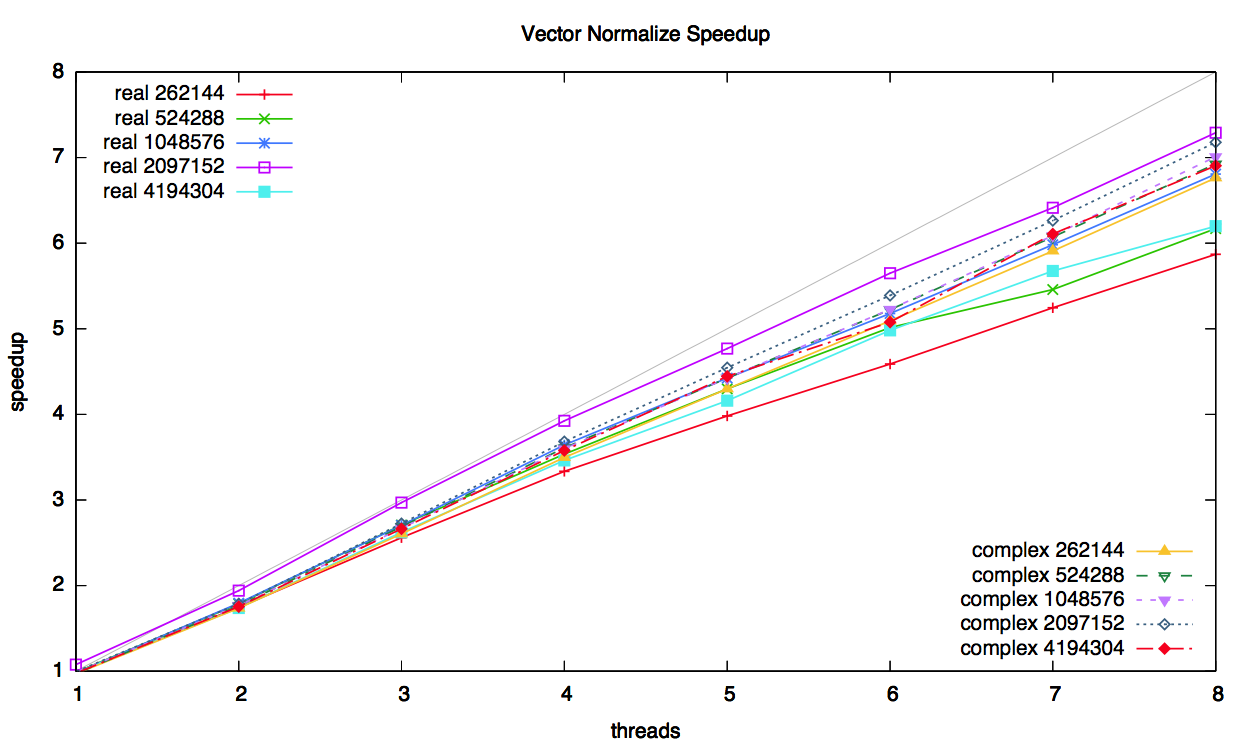
\includegraphics[width=1.09\columnwidth]{normalize.png}
	\caption{Speedup of normalizition of real and complex vectors of different sizes. The diagonal shows the ideal speedup.} \label{fig:normalize}
\end{figure}

\definition[Speedup.] As a basic performance metric of parallel performance, we define the speedup $S_p$ on $p$ processors as the ratio of the sequential execution time $T_1$ and the parallel execution time $T_p$.
\begin{equation}
S_p = {T_1 \over T_p}
\end{equation}
We call $S_p = p$ the \concept{ideal} or \concept{linear} speedup, occurring when a program scales perfectly with the number of processors. In practice, \concept{superlinear speedup} may occur; as the problem sizes for each processor diminish, more of the data can reside in the caches instead of main memory, speeding up memory access\cite{snyder-lin}. Note that in order to obtain a correct measure of speedup, accounting for parallel overhead, one must compare the parallel algorithm with the sequential algorithm, not just with the single-processor version of the parallel algorithm.
Plotting the speedup for different numbers of processors results in a speedup graph, obviously, this graph strongly depends on the specific problem and implementation.

\definition[Efficiency.] The efficiency $E_p$ of a program running on $p$ processors indicates the average efficiency of each processor.
\begin{equation}
E_p = {S_p\over p}
\end{equation}
An efficiency value of 1 corresponds to linear speedup. In general, the efficiency will amount to less than 1 and will diminish with the number of processors due to various sources of performance loss \cite{snyder-lin}.

\example We measure the speedup of the vector normalization algorithm above. Figure \ref{fig:normalize} displays the speedup graph for several vector sizes, overall showing a good result with efficiencies between 0.75 and 0.88.


\definition[Amdahl's Law.] Ultimately, the presence of non-parallellizable code limits the maximally attainable speedup of a program. If $s$ quantifies the total serial part of a program, then $1- s$ quantifies the total parallel part. Assuming perfect speedup of the parallel part, Amdahl's Law gives us an upper bound $\overline{S_p}$ on the total speedup
\begin{equation}
\overline{S_p} = \frac{T_1}{sT_1 + (1-s) {T_1 \over p}} = \left( s + {1 - s \over p} \right)^{-1}
\end{equation}
As the numbers of processors increases, the second term vanishes and $\overline{S_p} \to \sfrac{1}{s}$. Clearly, for a program with a negligible serial part, $\overline{S_p} \to p$ as $s \to 0$; we call such a program \concept{embarrassingly parallel}. Note that Amdahl's Law overestimates the upper bound in assuming limitless linear scaling of the parallel part.

\strongpar
While Amdahl's Law quantifies the influence of sequential bottlenecks in a program, it does not predict the actual parallel performance. As off-chip memory bandwidth constrains parallel performance of multicore programs and in particular of our application, we need a model to relate processor performance and memory traffic \cite{williams-waterman-patterson}.

\begin{figure}[ht]
	\centering
	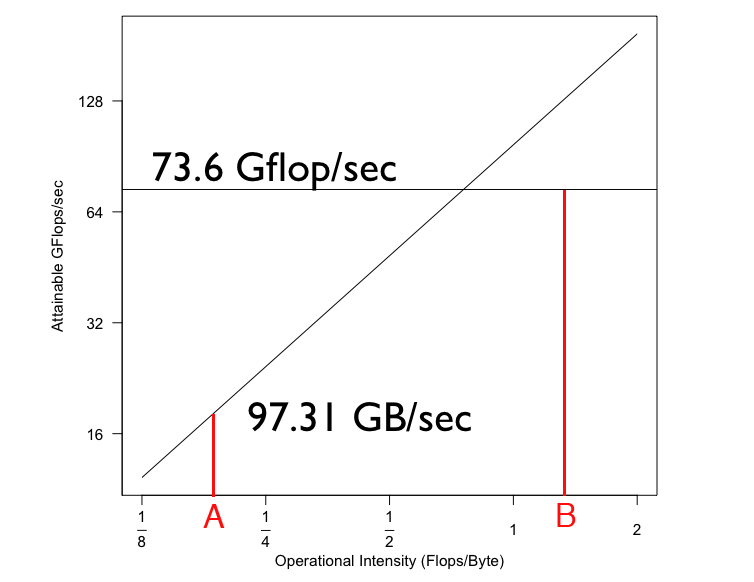
\includegraphics[width=0.9\columnwidth]{serenity-rooftop.png}
	\caption{Roofline characteristics of \code{serenity}, our testing machine \cite{serenity}. A memory-bound kernel $A$ hits the slanted part of the roof, a compute-bound kernel $B$  hits the flat part.} \label{fig:roofline}
\end{figure}
We use the therm \concept{operational intensity}, meaning the operations per byte of \acro{dram} traffic, as a measure of necessary \acro{dram} bandwidth needed by a kernel (the core computation) on a particular machine. The \concept{roofline} model, defined in \cite{williams-waterman-patterson}, relates floating-point performance, operational intensity, and memory performance of a machine in a 2D graph. For a kernel with a given operational intensity, peak performance coincides either with peak memory performance, in which case we call the kernel \concept{memory-bound}, or it coincides with maximal floating-point performance, which we call it a \concept{compute-bound} kernel. Optimally, a computational kernel would hit the intersection, meaning that it maximally uses both memory bandwidth and processor speed.


Like Amdahl's law, this model provides only an upper bound, however, the authors suggest a series of \concept{ceilings} an implementation must break through in order to achieve maximal performance. We will focus only on the memory bottlenecks, as our application will turn out strongly memory-bound due to a low operational intensity.
\begin{enumerate}
\item Optimizing for unit-stride memory access engages hardware prefetching, significantly reducing latency.
\item Ensure memory affinity, allocating memory and operating on data within the same memory-processor pair improves access times. This applies specifically to the \acro{numa} architecture of \code{serenity}.
\item Use software prefetching.
\end{enumerate}


\begin{figure}[hbt]
	\centering
	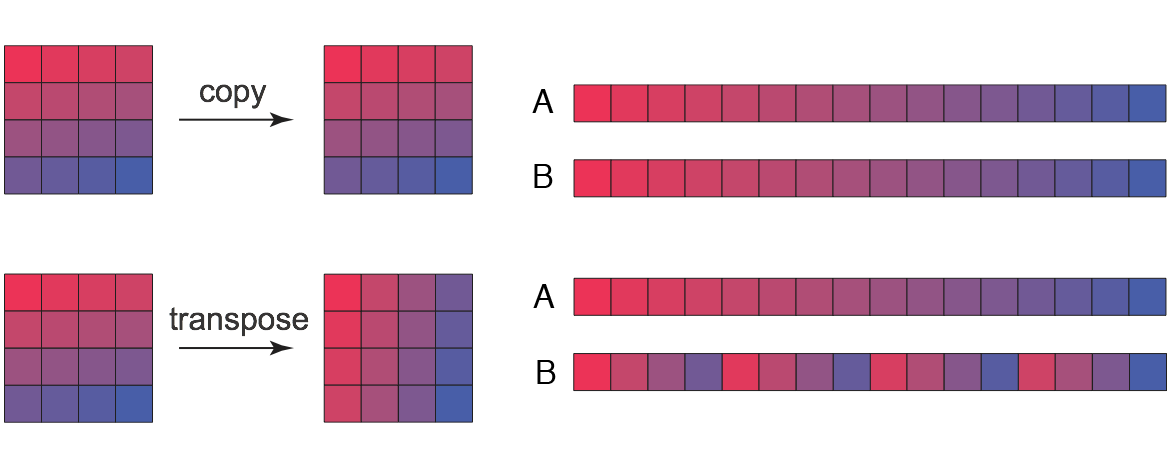
\includegraphics[width=\columnwidth]{transpose-cache.png}
	\caption{Transposition of a matrix in row-major storage format, compared to simple copying of the same matrix. Similar colours represent cache affinity.} \label{fig:transpose}
\end{figure}
\example As an example of a memory-bound algorithm, we implement a matrix transposition algorithm. Consider the naive (sequential) implementation to transpose a row-major matrix $A$ into a row-major matrix $B = A^\transpose$.
\lstinputlisting{transpose-naive.cpp}
Due to the row-major storage scheme, the reading of matrix $A$ uses unit stride, but the writing of $B$ does not, as illustrated in Figure \ref{fig:transpose}.


To make better use of the caches and hardware prefetching, we will implement an algorithm based on the scheme presented by Frigo et al.\cite{frigo} For simplicity, we will limit ourselves to $n \times n$ (square) matrices, where $n = 2^k$ with $k$ a non-negative integer. For a matrix $A$ containing four submatrices $A_i$, we have
\begin{equation*}
\begin{split}
A^\transpose = \mat{A_1 & A_2 \\ A_3 & A_4}^\transpose &= B \\
\mat{A_1^\transpose & A_3^\transpose \\ A_2^\transpose & A_4^\transpose}  &= \mat{B_1 & B_2 \\ B_3 & B_4}
\end{split}
\end{equation*}
This relation suggests a divide and conquer approach: if we recursively divide $A$ and $B$ in four blocks, we will arrive at a point where, in principle, a source block from $A$ and its corresponding destination block in $B$ could fit in the cache. Copying the elements from the $A$ block to the $B$ block can then happen in an arbitrary order. Hence, we can simply continue splitting recursively, up to blocks of unit size, ignorant of when the blocks become small enough to fit in the cache. We call this approach \concept{cache-oblivious}, as we don't need any details regarding the cache or cache-line size and yet obtain an implementation that uses the caches effectively.


\begin{figure}[hbt]
	\centering
	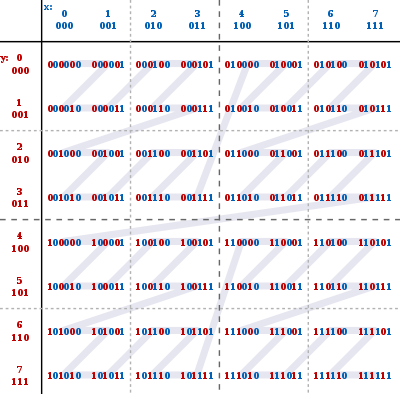
\includegraphics[width=0.8\columnwidth]{z-order.png}
	\caption{Z-order traversal of a matrix \cite{wiki-z-order}.} \label{fig:z-order}
\end{figure}
To avoid recursive function calls, we will use a \concept{Z-order}\footnote{sometimes called \concept{Morton order}} traversal of the matrix, illustrated in Figure~\ref{fig:z-order}. For an element of matrix $A$ at row $i$ and column $j$, we find the Z-value by interleaving the binary representations of $i$ and $j$. The reverse operation, deinterleaving, turns a Z-value into a row and column index. By definition, the Z-order traversal results in the recursive block structure described above. Note that compared to the naive implementation, the divide and conquer method executes the same data movements (\code{B[j][i] = A[i][j]}), all we did was change the order of the operations.
\lstinputlisting{transpose-dc.cpp}


We omit the parallel transpose adaptations\footnote{The source code at \url{http://github.com/kmoerman/pqvm} contains the straightforward yet verbose parallel versions of both the naive and the divide and conquer methods.}, as the sequential version already captures the essence. Figure~\ref{fig:transpose-speedup} displays the speedup results. Note that superlinear scaling occurs for the smaller matrices, as they still fit perfectly in cache memory. For the larger matrices of 2048 by 2048 and 4096 by 4096 \code{double} elements, the divide and conquer method clearly scales better, with efficiencies of about 1, compared to the naive efficiency of about 0.38.
\begin{figure}[hb]
	\centering
	\hspace*{-0.07\columnwidth}
	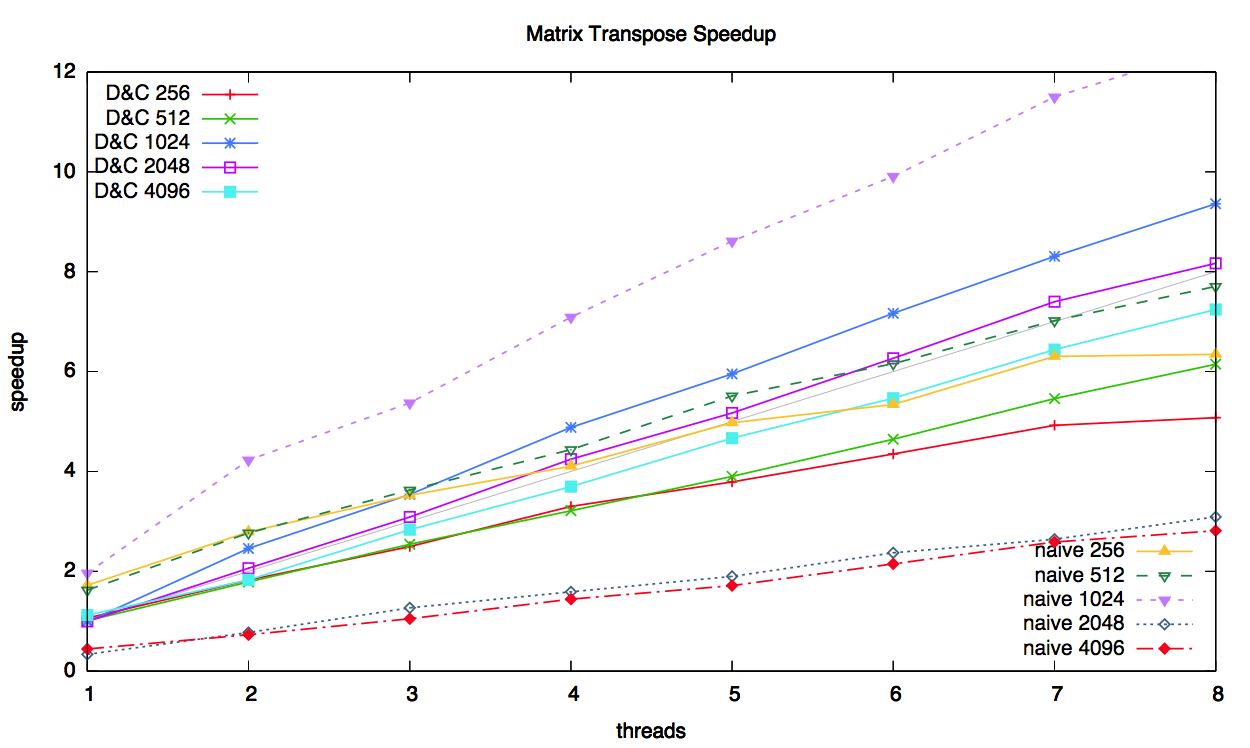
\includegraphics[width=1.09\columnwidth]{transpose.png}
	\caption{Matrix transpose using a naive and a divide and conquer algorithm for square matrices of different sizes.} \label{fig:transpose-speedup}
\end{figure}


\strongpar
If we want to match the metrics introduced above with an actual implementation, we need methods of analyzing our code and the resulting program. The \code{libpapi} library \cite{libpapi} provides some performance analysis functions for accessing hardware counters, which we must manually include in the code. We provide a header file \code{performance.h} wrapping some of the functionality, which we use in some of our profiling programs, to select specific parts we want to measure.

The \code{perf} tools, a collection of profiler tools, periodically interrupts a running program to collect hardware counters and call-stack info, this allows for less obtrusive measuring of the codes performance. We use the command \code{perf stat} to quickly assess run time behaviour (running times, cache misses, \acro{cpu} workload). With \code{perf record}, one can record events during the execution of a program; \code{perf report} provides an interface for analyzing the recorded events, \code{perf annotate} supplies the source code with counted events (function calls, cache misses, etc.) \cite{perf}.



%% CHAPTER VIRTUAL MACHINE
\chapter{Implementing the Virtual Machine}\label{chp:implementation}
We can now expose the work on \code{pqvm}, our implementation of the execution layer of the quantum programming framework introduced in the first chapter. We developed the mathematical model for the basic operations in \acro{mc} in Chapter \ref{chp:qop-mc}, from which we can derive our implementation, following the guidelines set out in Chapter \ref{chp:platform}. A \code{Git} repository on \url{https://github.com/kmoerman/pqvm} contains the full source code\footnote{Actually, the code can serve as a self-explanatory document on its own and contains extra implementation details that would otherwise needlessly obfuscate this report.}, we will only include the parts relevant to this document. To avoid the verbosity of \code{TBB} code, we will use pseudo \code{C++} code, especially \code{\bfseries parallel for} loops, unless the exact parallel implementation requires scrutiny.


\section{Dense State Vectors}
The \code{libquantum} backend of \code{qvm}, the existing sequential \acro{vm}, uses a sparse state vector implementation, saving memory by omitting the zero valued amplitudes. While bringing down the memory footprint, this approach leads to poor cache usage, resulting in a bad overall memory performance. This bottleneck corresponds to the first performance ceiling memory-bound applications must break trough (see Chapter~\ref{chp:platform}). We will implement dense state vectors to improve cache usage by allowing unit stride access of a quregister. We implement both a sequential and a parallel \acro{vm}, using the sequential version as a reference for speedup measurements. In this report, we include only a part of the implementation, as much of the operators share a similar structure and behaviour.


\paragraph{State vector} We write our own \code{STL}-style vector class (see \code{vector.h}), as the classic \code{std::vector} class provides now way of allocating space before filling the vector concurrently. We define the \code{quregister} type as a \code{vector} of \code{std::complex <double>} numbers, the amplitudes of the quantum state.
At index \code{i} of the vector, we store the amplitude $\alpha_i$ belonging to the computational basis state $\ket i$.


\paragraph{Tangle} As we trade off memory for speed, the memory footprint of our implementation will inevitably increase compared to the original \code{qvm}. In general, a quregister of $n$ qubits requires storing $2^n$ amplitudes, however, we retain an important optimization from the original implementation. When we decompose a quantum state as a tensor product of substates, we can effectively reduce the exponential factor and consequently the memory footprint. In fact, we do not even need to find the tensor decomposition of arbitrary state vectors, the small set of operations and the explicit entanglement operator allow us to keep track of the entangled and disentangled parts of the simulated quantum system. Thus, we split the entire quantum state space into disjoint parts called \concept{tangles}. In the implementation, a \code{tangle} stores a lists of the qubits it contains and a state vector of the quantum system it represents.

Whenever the entanglement operator entangles two qubits residing in different tangles, we merge the tangles using the tensor product. As the measurement of a qubit entails its destruction, a tangle shrinks when the measuring one of its qubits; removing a qubit from a quantum state halves the number of stored amplitudes.

\paragraph{Kronecker product} The kronecker product merges two quantum states (i.e. tangles), in accordance with Postulate~\ref{thm:post-compose}. We split the parallel range along the left input vector; each task writes to its own contiguous part of the result vector and we obtain unit stride access for the right input vector and the result vector.
\lstinputlisting{kronecker.cpp}


\paragraph{X operator} Recall from Chapter \ref{chp:qop-mc} that applying the $X_{n-k}$ operator on the basis vectors of a state space of $n$ qubits will map $k$-even indices $i$ to $i + 2^k$ and $k$-odd indices $j + 2^k$ to $j$, therefore, we simply need to exchange the amplitudes of $k$-odd and $k$-even indices. However, instead of implementing these exchange operations directly, the periodic behaviour of $\parity_k$ allows us to perform block transfers
Thus, we implement the $X_t$ operator in three steps: allocate a new state vector, then copy the even blocks and, finally, copy the odd blocks. Consider the (simplified) parallel implementation of the even step
\lstinputlisting{sigma-x.cpp}
\code{TBB}'s \code{parallel\_for} will split the input state vector in ranges and assign an \code{x\_even} task to each range. We then calculate the number of periods in the range and call \code{memcpy} to perform the data transfer of each even block.


\paragraph{Z operator} The $Z_t$ operator negates every odd-indexed amplitude. This task object iterates the amplitudes in a given range of the input vector and negates the odd-indexed amplitudes, skipping the even ones. To show the importance of data movement, we first show a version that copies the input vector while applying $Z$, in the next section we do away with the unnecessary copy.
\lstinputlisting{sigma-z1.cpp}

\section{In Place Operations}
While we cannot turn $X$ into an in place operation, however, we can do so with $Z$ and $\widehat{Z}$. Further reducing the workload will show a great performance benefit. The code below implements the  $Z$ operator transforming only the odd blocks.
\lstinputlisting{sigma-z2.cpp}

\paragraph{Controlled Z operator} The $\widehat{Z}_{c,t}$ operator applies $Z_t$ to odd basis vectors (basis vector with a control qubit in state $\ketb{1}$). The implementation resembles the $Z$ operator, with one extra \code{for} nesting; for brevity we present only the in-place version.
\lstinputlisting{control-z.cpp}


\section{Experimental Results}
\paragraph{Individual operators} We first present the speedup results of the individual operators. Each operator was executed 5 times, on random vectors of 20 qubits ($2^20$ complex amplitudes), allowing for ample parallelism. We only measure the time for the actual operation, the initialisation of the input state has no influence.

\begin{figure}[hbp]
	\centering
	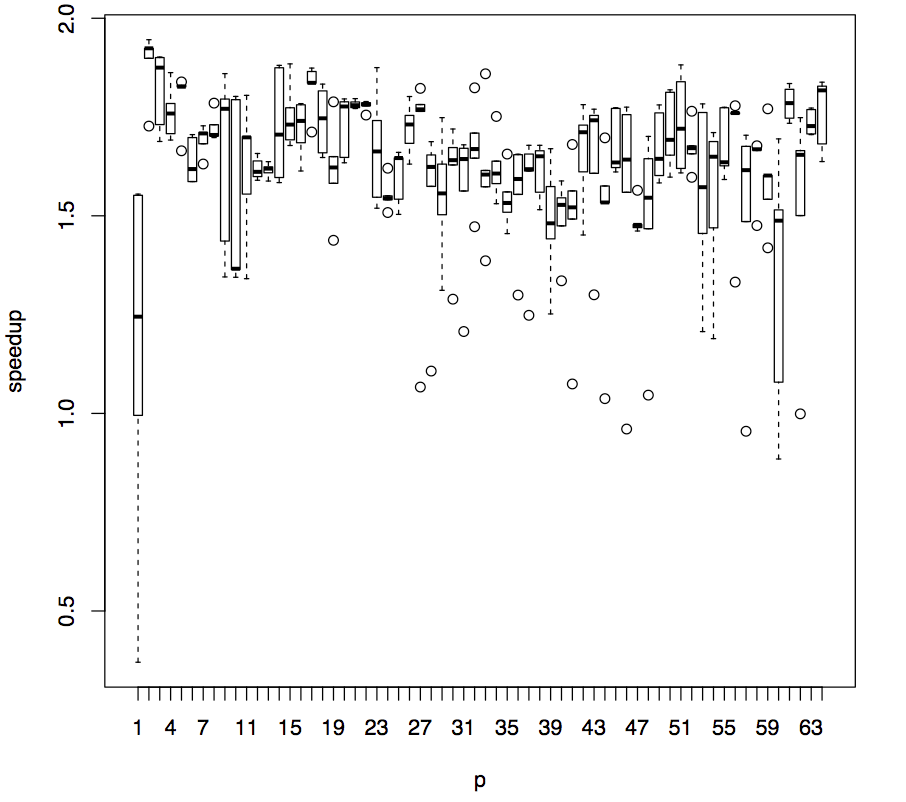
\includegraphics[width=\columnwidth]{kronecker.png}
	\caption{Speedup of the kronecker product. We observe no actual scaling beyond 4 processors.}
\end{figure}

\begin{figure}[p]
	\centering
	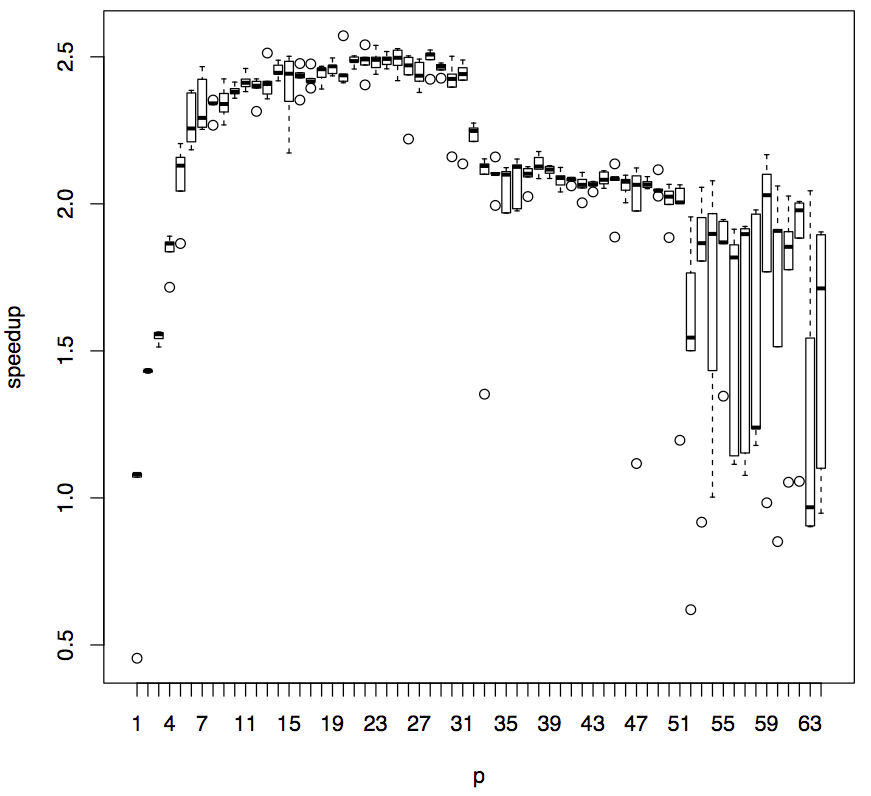
\includegraphics[width=\columnwidth]{sigma-x.png}
	\caption{Speedup of the $X$ operator. $X$ exhibits sublinear scaling, which halts beyond 8 processors.}
\end{figure}

\begin{figure}[p]
	\centering
	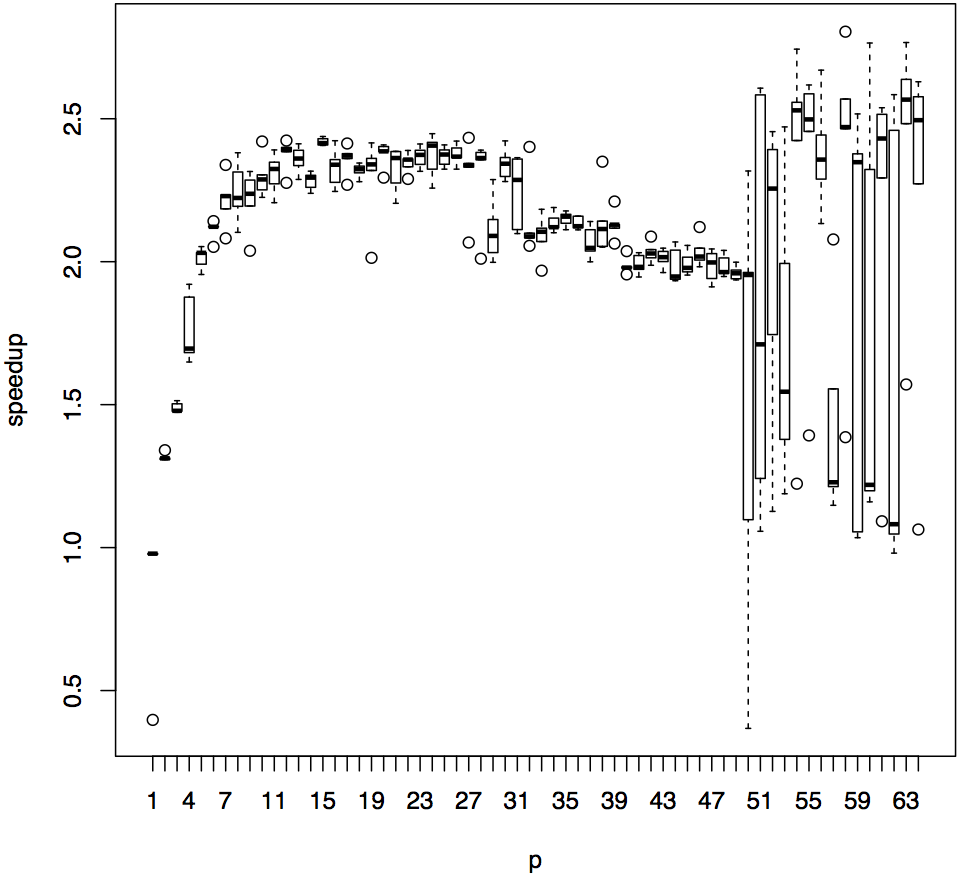
\includegraphics[width=\columnwidth]{sigma-z1.png}
	\caption{Speedup of the copying $Z$ operator. The scaling behaviour of $Z$ resembles that of $X$.}
\end{figure}

\begin{figure}[p]
	\centering
	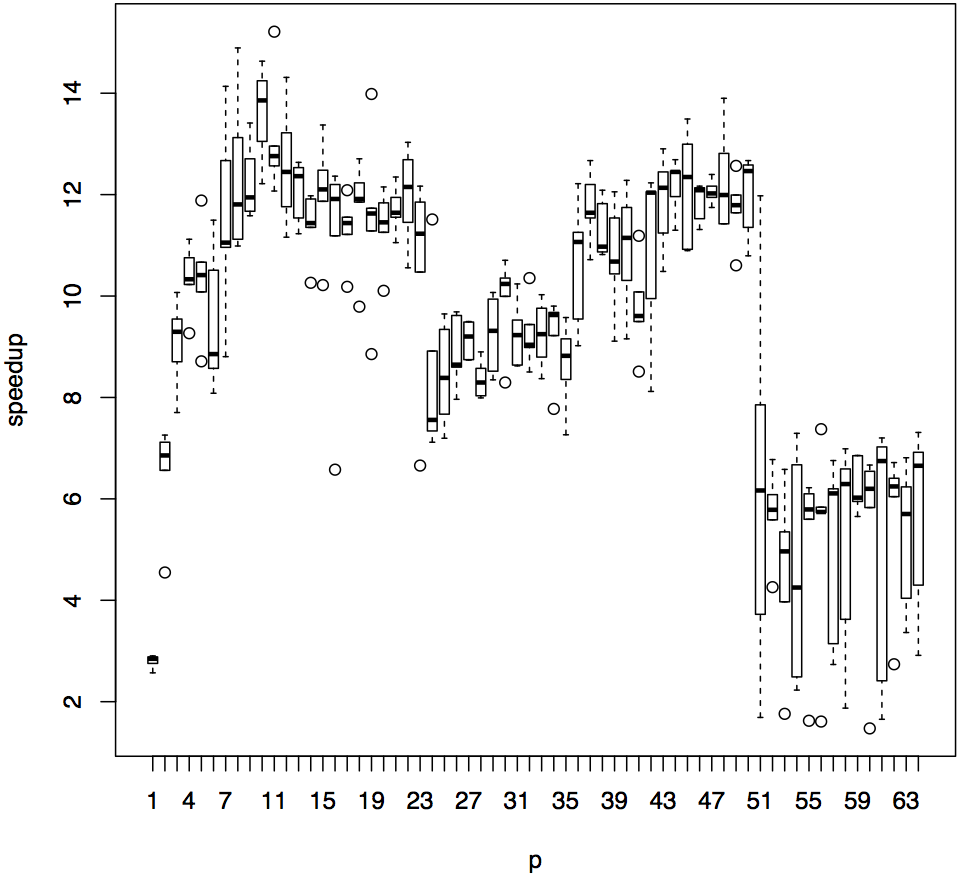
\includegraphics[width=\columnwidth]{sigma-z2.png}
	\caption{Speedup of the in-place $Z$ operator. This version shows larger speedup, but again scaling stops beyond 8 processors.}
\end{figure}

\begin{figure}[p]
	\centering
	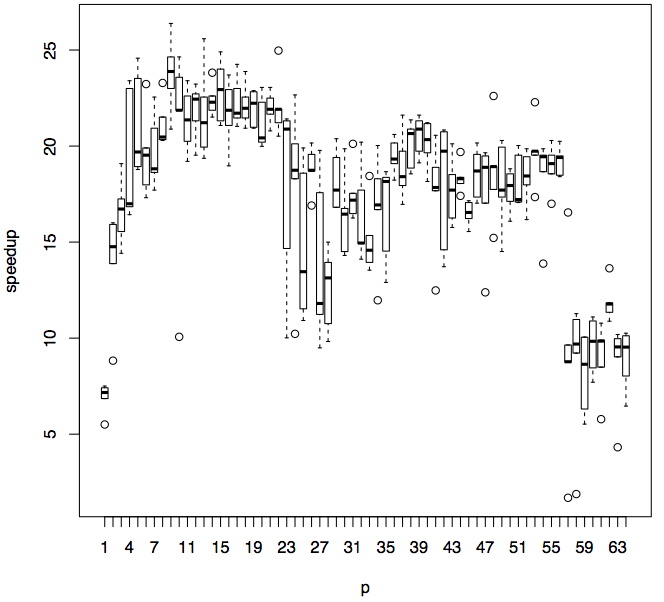
\includegraphics[width=\columnwidth]{control-z.png}
	\caption{Speedup of the in-place $\widehat{Z}$ operator, similar the the $Z$ operator.}
\end{figure}

\clearpage
\paragraph{Performance of pqvm.} Next, we show the combined effect of these operations in \code{pqvm}. As a benchmark, we run \code{qft16}, a quantum fourrier transform of 16 qubits, the same benchmark used for testing the sequential version in \cite{vandriessche}. Again we see no improvement beyond 8 processors. An inspection with \code{perf} on the $X$ operator (Fgure \ref{fig:perf-x}), shows that execution spends the majority of its time in the actual tasks, with little overhead from \code{TBB}\footnote{With similar results for the other operators, not included for brevity.}. However, when we look at the execution of \code{pqvm} as a whole (Figure \ref{fig:perf-pqvm}), we see a majority of the time spent in the \code{TBB} runtime (\code{libtbb.so.2}).
\begin{figure}[hbp]
	\centering
	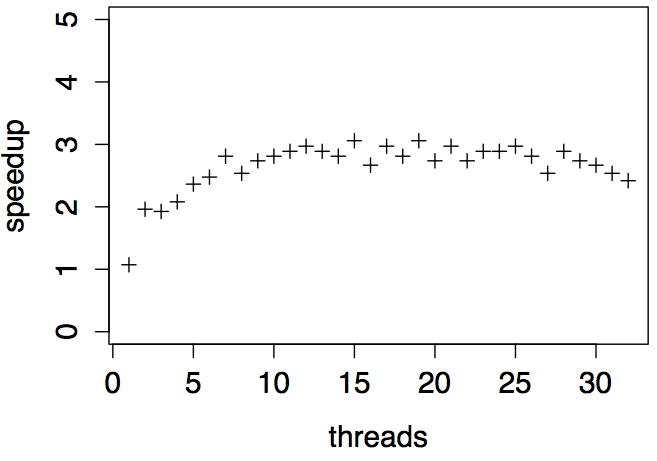
\includegraphics[width=\columnwidth]{pqvm-speedup.png}
	\caption{Speedup of the entire \code{pqvm} program,up to 32 processors. The shape of this graph follows the general behaviour observed in the previously shown experiments.}
\end{figure}

\begin{figure}[hbp]
	\centering
	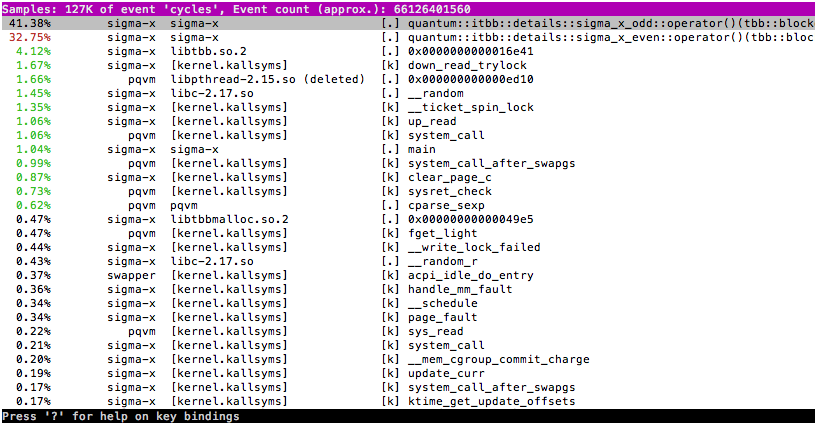
\includegraphics[width=\columnwidth]{perf-sigma-x.png}
	\caption{The \code{perf} sampling of \code{X}; 74\% time in the actual tasks \code{sigma\_x\_even} and \code{sigma\_x\_odd}.}\label{fig:perf-x}
\end{figure}

\begin{figure}[hbp]
	\centering
	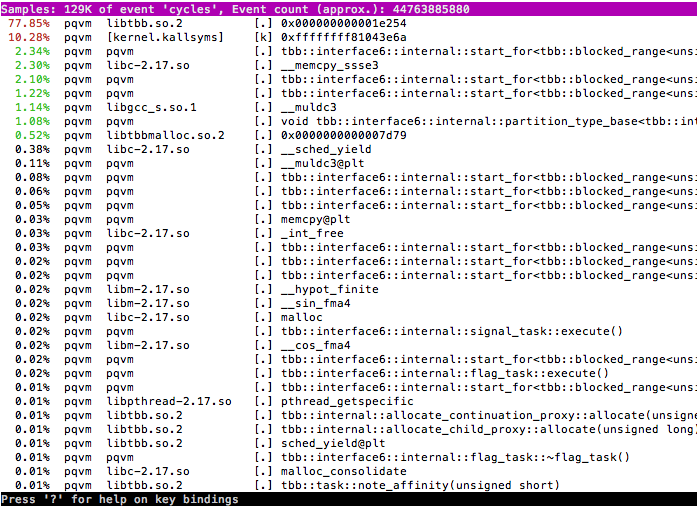
\includegraphics[width=\columnwidth]{perf-pqvm.png}
	\caption{The \code{perf} sampling of \code{pqvm} running \code{qft16}; 77\% of time in the \code{TBB} runtime}\label{fig:perf-pqvm}
\end{figure}

\paragraph{Overall result} We now present the overall result of our project, the speedup of the final parallel implementation compared to the original sequential implementation. Measured with \code{GNU time}, running the \code{qft16.mc} benchmark, \code{qvm} takes 4.333 seconds; \code{pqvm} in sequential mode takes 1.206 seconds; \code{pqvm} running on 8 threads takes 0.405 seconds.

%% CHAPTER CONCLUSIONS
\chapter{Conclusions and Future Work}
The dense state vectors and efficient cache usage turn out as our main result. While our implementation proves no match for a complex machine like \code{serenity}, the results indicate that an implementation on smaller multicore machines (2, 4, 8 cores) can produce a reasonable speedup.

As \code{TBB} exhibits a high overhead, we might opt for another library in future implementations. The current memory model (large state vectors) seems unfit for \acro{numa} machines; it might turn out better to split the quantum state across the nodes, and have each node operate mainly on its own part. However, as \code{TBB} hides the actual threads (and therefore the nodes and processors) in smaller grained tasks, other libraries (\code{ArBB} for instance) seem better suited.

As a hybrid between an interpreter and a compiler approach, we propose a deferred execution approach, grouping the execution of multiple operators into one; this would increase operational intensity, performing more on-chip work per byte of data, thus shifting the interpreter towards the roofline optimum. Furthermore, instead of storing each amplitude at an index corresponding to its basis state, we could easily store the basis state with along with it, yielding more numerical transformations and fewer data movement! Apart from the obvious gain in execution speed, we claim that such a model would work for sparse states as well, without losing unit stride access (note that we have never required random access). This claim needs more time and effort than we had available, however, it still seems within reach, given our current understanding of quantum simulation.

\strongpar
{\it Finally, I would like to offer a word of thanks to my advisor Yves Vandriessche, for the many hours he has spent teaching and assisting me the past year.}

\clearpage
\raggedright
\bibliographystyle{plain}
\nocite{*}
\addcontentsline{toc}{chapter}{Bibliography}
\bibliography{bachelorproef}


\end{document}